% Provenance (never printed): old terminale S material on the disappearance of
% mountain ranges (erosion, transport, sedimentation, isostatic rebound, the
% recycling of continental material). Owner (Sync 0/1): denudation rate,
% sediment load (bed, suspended, dissolved), isostatic rebound, detrital rock,
% diagenesis. Weathering, erosion, deposition are Book 1's (g5); hydrolysis and
% clay minerals g10.07's; discharge g10.08's; isostasy and Airy's model g11.03's;
% sedimentary basin g11.09's; mountain root g12.01's; metamorphism g12.03's;
% half-life is physics' (recalled in prose). Figures: figdata/grade-12/relief_decay.py
% (rates, decay curves, the Varden unconformity from figdata/shared/region.py).
\chapter{The Destruction of Mountains}\label{ch:g12:destruction-of-mountains}

Seen from the International Space Station, the Appalachian Mountains of
eastern North America are a striking pattern of long, dark, forested ridges
and pale farmed valleys, more than \qty{500}{km} of them in the photograph
below. The ridges are hard rock layers that were crumpled into tight \omterm{def:g12:mountain-building:fold}{folds}
when Africa pushed against North America, in the Carboniferous and Permian
periods, more than 250 million years ago. Today their highest summit, Mount
Mitchell, the highest point east of the Mississippi River, stands
\qty{2037}{m} above sea level, less than a quarter of the height of Everest.
% ledger: photo:g12-appalachians, usgs:alleghanian, usgs:alleghanian-age, ics:base.Triassic, ncparks:mitchell (6684 ft), tht:everest (Book 1 row, 8848.86 m)

\begin{omfigure}
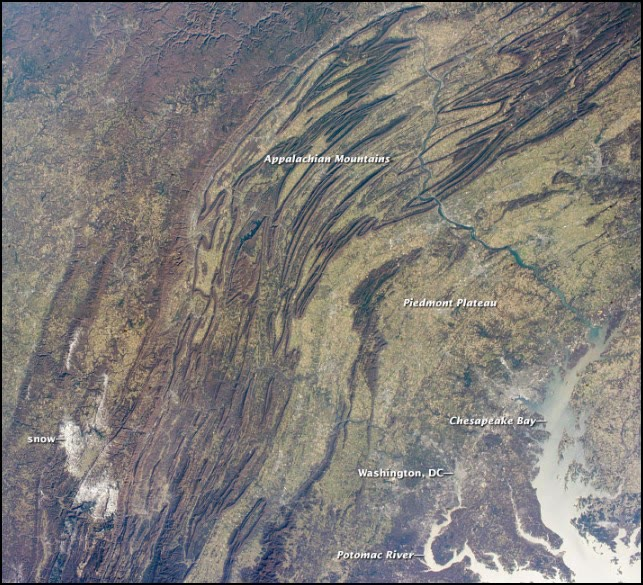
\includegraphics[width=0.6\linewidth]{images/book2/g12-iss-appalachians.jpg}

{\small The valley-and-ridge Appalachians, from north-eastern Pennsylvania
(top right) to West Virginia, photographed from the International Space
Station on 17 November 2012. The forested ridges are hard rock layers, the
farmed valleys softer ones. Photograph NASA (public domain).}
\end{omfigure}
% ledger: photo:g12-appalachians

A mountain range does not last. From the moment it rises, rain, ice and
rivers attack it; the rock they carry away ends up in the sea, where it
becomes new rock. This chapter measures how fast that happens, follows the
debris to the place where it turns to stone, and shows why a range that is
being worn down keeps rising as it goes.

\begin{recall}
Weathering breaks rock down where it stands; erosion carries the debris away
and deposition lays it down elsewhere (Book 1, grade 5). \omterm{def:g10:soil-formation:chemical-weathering}{Chemical weathering}
turns feldspars into \omterm{def:g10:soil-formation:clay}{clay minerals} by \omterm{def:g10:soil-formation:hydrolysis}{hydrolysis}
(\cref{ch:g10:soil-formation}). The \omterm{def:g10:drainage-basins:discharge}{discharge} of a river is the volume of
water that passes a point in a second (\cref{ch:g10:drainage-basins}). The
crust floats on the mantle in \omterm{def:g11:lithosphere-asthenosphere:isostasy}{isostasy}; in Airy's model, a region whose crust
is thicker by $\Delta H$ stands higher by $\Delta H\,(\rho_m - \rho_c)/\rho_m$
(\cref{ch:g11:lithosphere-asthenosphere}), and a high range rests on a \omterm{def:g12:continental-crust:root}{root}
of thick crust (\cref{ch:g12:continental-crust}). Sediments accumulate in
\omterm{def:g11:fossil-fuel-geology:basin}{sedimentary basins} (\cref{ch:g11:fossil-fuel-geology}). Rocks buried deep in
a mountain belt are metamorphosed (\cref{ch:g12:metamorphic-rocks}).
\end{recall}

\section{How fast is the land worn down?}

\begin{definition}[Denudation rate]\label{def:g12:destruction-of-mountains:denudation}
The \emph{denudation rate}\index{denudation rate} of a region is the mean
thickness of rock that weathering and erosion together remove from it per
unit of time. It is usually given in metres per million years
(\unit{m/Myr}), which is the same as millimetres per thousand years.
\end{definition}
% ledger: pb11:rates (rates in m/Myr), earle:loads

How can one measure something so slow? Cosmic rays striking the ground make
a rare isotope, beryllium-10, in the quartz of the top few metres of rock.
The slower a surface is worn down, the longer each grain stays near the top,
and the more beryllium-10 it gathers. Measuring it in the sand of a river
gives the mean \omterm{def:g12:destruction-of-mountains:denudation}{denudation rate} of the whole basin upstream, over the last
thousands to millions of years.
% ledger: pb11:rates (10Be produced within a few metres of the surface; concentration reflects near-surface residence time; 10^3 to 10^6 years)

A compilation of 1599 such measurements found that bare rock outcrops are
worn down slowly, by \qty{12}{m/Myr} on average (median
\qty{5.4}{m/Myr}), and never faster than \qty{140}{m/Myr}. Whole \omterm{def:g10:drainage-basins:drainage-basin}{drainage
basins} lose much more, \qty{218}{m/Myr} on average, but with a median of
only \qty{54}{m/Myr}: a few fast basins pull the mean up. The fastest are
the steep ones: the mean slope of a basin is the factor that best predicts
its rate. Basins in seismically active regions, where mountains are rising,
erode about twice as fast as those in quiet regions.
% ledger: pb11:rates

\begin{omfigure}
\begin{tikzpicture}
\begin{axis}[omrecord, xbar, xmode=log, log origin=infty, bar width=7pt, bar shift=0pt,
  width=0.62\linewidth, height=6.6cm, scale only axis, xmin=3, xmax=1000,
  ymin=0.4, ymax=10.6, ytick={1,...,10}, y tick label style={font=\scriptsize, align=right},
  yticklabels={{outcrops, median}, {outcrops, mean}, {world rivers (budget)}, {basins, median},
    {Mississippi, before 1900 (budget)}, {arid basins, mean}, {quiet basins, mean}, {basins, mean},
    {seismically active basins, mean}, {polar basins, mean}},
  xlabel={denudation rate (\unit{m/Myr}), logarithmic scale}, ymajorgrids=false,
  unbounded coords=discard, nodes near coords, nodes near coords align={horizontal}, nodes near coords style={font=\scriptsize},
  point meta=rawx, every node near coord/.append style={/pgf/number format/.cd, fixed, precision=0}]
% computed in figdata/grade-12/relief_decay.py; ledger: pb11:rates, mm10:mississippi, kammerer:mississippi, earle:loads, cm95:crust
\addplot[fill=omThm!45, draw=omThm, every node near coord/.append style={/pgf/number format/.cd, fixed, precision=1}] table[x=measured, y=idx] {figdata/out/grade-12-relief_decay-rates.dat};
\addplot[fill=omDef!45, draw=omDef] table[x=budget, y=idx] {figdata/out/grade-12-relief_decay-rates.dat};
\end{axis}
\end{tikzpicture}

{\small \omterm{def:g12:destruction-of-mountains:denudation}{Denudation rates} measured with beryllium-10 (red: 1599 measurements,
1149 of them in river sand) and two rates computed in this chapter from the
sediment that rivers carry (blue). Sources: Portenga and Bierman (2011);
Meade and Moody (2010); Syvitski and others (2005).}
\end{omfigure}
% values: world_m_per_myr 43.5, miss_before_1900_m_per_myr 51.6 (relief_decay.py)

\section{Rivers carry the mountains away}

Much of what is worn off the land leaves it in rivers.

\begin{definition}[Sediment load]\label{def:g12:destruction-of-mountains:load}
The \emph{sediment load}\index{sediment load} of a river is the material it
carries, in three forms: the \emph{bed load}\index{bed load}, large grains
rolled, pushed or bounced along the bottom; the \emph{suspended
load}\index{suspended load}, small grains held up in the moving water; and
the \emph{dissolved load}\index{dissolved load}, ions in solution, such as
calcium and chloride, left by \omterm{def:g10:soil-formation:chemical-weathering}{chemical weathering}.
\end{definition}
% ledger: earle:loads

On average, the \omterm{def:g12:destruction-of-mountains:load}{dissolved load} is about \qty{15}{\percent} of the mass a
river carries. The faster the water, the larger the grains it can lift. A
sand grain \qty{1}{mm} across is picked up from the bed at about
\qty{20}{cm/s}, and once moving it stays in suspension until the current
falls below \qty{10}{cm/s}. Silt grains are harder to lift than sand,
because they stick together: a grain of \qty{0.01}{mm} needs
\qty{60}{cm/s} to be picked up, but then a current of \qty{0.1}{cm/s} keeps it
in suspension. That is why rivers in flood run brown, and why the finest mud
travels all the way to the sea.
% ledger: earle:loads

\begin{omfigure}
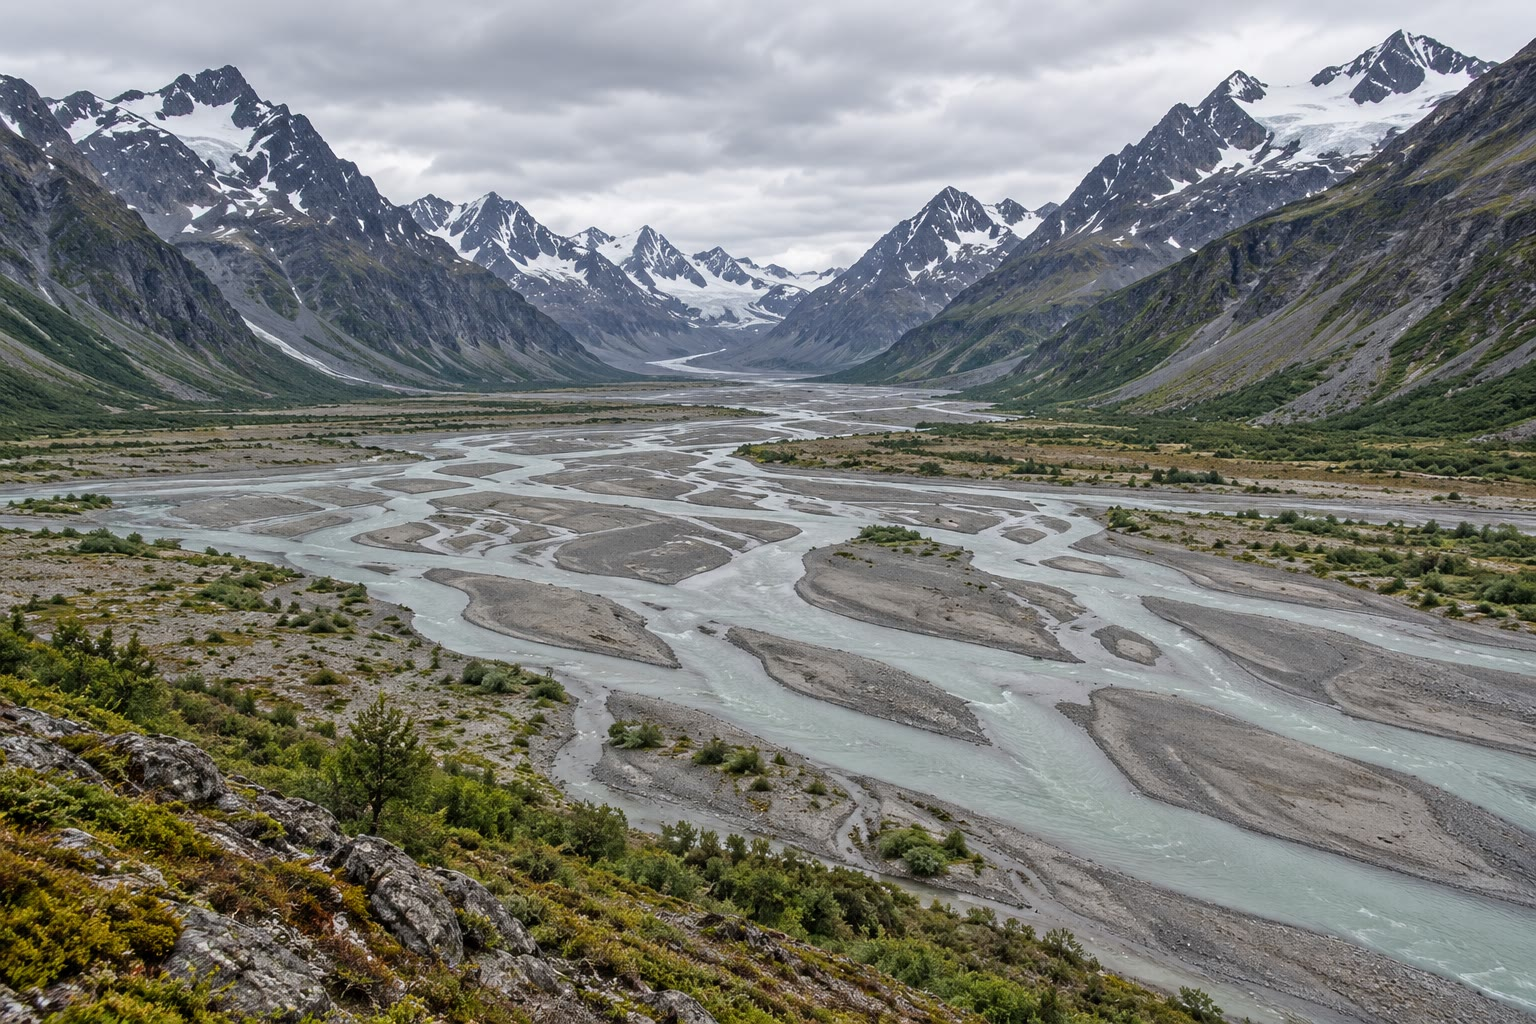
\includegraphics[width=0.66\linewidth]{images/book2/ai/g12-braided-river.jpg}

{\small A braided river in a glacial mountain valley: shallow channels split
and rejoin between bars of gravel that the water moves only in floods.
AI-generated illustration.}
\end{omfigure}

Measuring what a river carries gives a second way to find a \omterm{def:g12:destruction-of-mountains:denudation}{denudation rate}.

\begin{method}[An erosion budget]\label{met:g12:destruction-of-mountains:budget}
\begin{enumerate}
  \item Take the mass of sediment the river carries in a year, and add the
        \omterm{def:g12:destruction-of-mountains:load}{dissolved load} (if only the solid load is known, divide it by
        $0.85$).
  \item Divide by the density of the rock, about \qty{2830}{kg/m^3} for the
        \omterm{def:g12:continental-crust:continental-crust}{continental crust}, to get the volume of rock removed each year.
  \item Divide by the area of the \omterm{def:g10:drainage-basins:drainage-basin}{drainage basin}: this is the thickness
        removed each year.
  \item Multiply by $10^6$ to express it in metres per million years.
\end{enumerate}
\end{method}
% ledger: earle:loads, cm95:crust

\begin{example}[The Mississippi]\label{ex:g12:destruction-of-mountains:mississippi}
Before 1900, the Missouri--Mississippi river system carried about 400
million tonnes of sediment a year to the sea, from a basin of about
\qty{2980000}{km^2}. With the \omterm{def:g12:destruction-of-mountains:load}{dissolved load}, $400/0.85 \approx 471$ million
tonnes, that is $\num{4.71e11}/2830 \approx \qty{1.66e8}{m^3}$ of rock a year.
Spread over $\qty{2.98e12}{m^2}$, it is a layer
\[
  \frac{\num{1.66e8}}{\num{2.98e12}} \approx \qty{5.6e-5}{m}
  \text{ a year, about } \qty{56}{m/Myr}.
\]
Between 1987 and 2006 the river carried only 145 million tonnes a year, which
gives about \qty{20}{m/Myr}: dams built on the Missouri in the 1950s trap
about 100 to 150 million tonnes a year, and other works hold back more.
\end{example}
% ledger: mm10:mississippi, kammerer:mississippi, earle:loads, cm95:crust
% values: miss_before_1900_m_per_myr 55.8, miss_1987_2006_m_per_myr 20.2 (relief_decay.py)

The same budget can be made for the whole world. Before people changed the
rivers, they carried about 15.5 billion tonnes of solid sediment a year to
the coasts; with the \omterm{def:g12:destruction-of-mountains:load}{dissolved load}, that is about \qty{6.4}{km^3} of rock a
year, taken from the \qty{1.48e8}{km^2} of the continents: a mean \omterm{def:g12:destruction-of-mountains:denudation}{denudation
rate} of about \qty{43}{m/Myr}, close to the median of the beryllium-10
measurements. People have since changed both terms: soil erosion has
increased what rivers pick up by about 2.3 billion tonnes a year, but more
than 100 billion tonnes of sediment now lie behind dams.
% ledger: syvitski:modern-flux (Book 1 row, prehuman 15.5 Gt/yr with bed load), sy05:humans, data:etopo1 (land fraction 0.290, grade-11 hypsometry), cm95:crust
% values: world_volume_km3_per_yr 6.44, land_area_km2 1.48e8, world_m_per_myr 43.5 (relief_decay.py)

\section{From sediment to rock}

What the rivers carry is laid down where the current slows: in valleys and
lakes, on deltas, and above all in the \omterm{def:g11:fossil-fuel-geology:basin}{sedimentary basins} of the continental
margins. Layer after layer, the sediment is buried, and it slowly turns to
rock.

\begin{definition}[Detrital rock; diagenesis]\label{def:g12:destruction-of-mountains:diagenesis}
A \emph{detrital rock}\index{detrital rock} (or clastic rock) is a
sedimentary rock made of fragments, the clasts, of older rocks and minerals.
\emph{Diagenesis}\index{diagenesis} is the set of changes that turn a buried
sediment into rock at low temperature: \emph{compaction}, as the weight of
the layers above squeezes out water and air, then \emph{cementation}, as
minerals that crystallise from the water in the pores (calcite, quartz,
hematite, \omterm{def:g10:soil-formation:clay}{clay minerals}) glue the grains together.
\end{definition}
% ledger: earle:clastic

\omterm{def:g12:destruction-of-mountains:diagenesis}{Detrital rocks} are named by the size of their clasts:
\begin{itemize}
  \item a \textbf{conglomerate} is made of rounded clasts larger than
        \qty{2}{mm}, a \textbf{breccia} of angular ones;
  \item a \textbf{sandstone} is made of sand, grains between \qty{2}{mm}
        and \qty{0.063}{mm}, most often of quartz, the mineral that best
        resists weathering;
  \item a \textbf{mudrock} holds at least \qty{75}{\percent} silt and clay;
        it is a shale if it splits into thin layers.
\end{itemize}
% ledger: earle:clastic

\begin{omfigure}
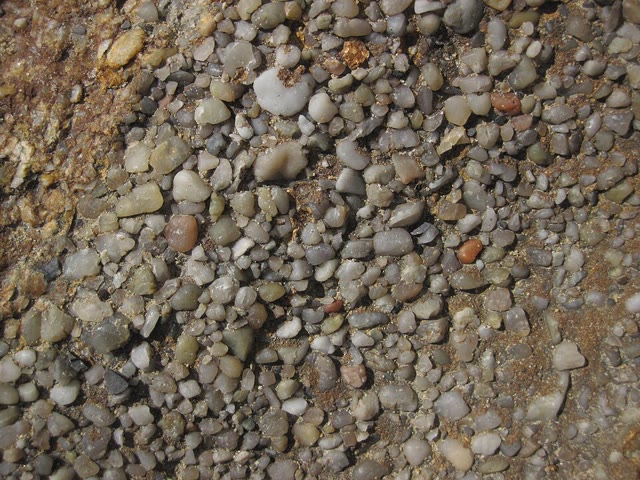
\includegraphics[width=0.5\linewidth]{images/book2/g12-stjohn-conglomerate.jpg}

{\small A quartz-pebble conglomerate from Ohio, of Carboniferous age:
rounded pebbles of quartz, cemented by finer sand. Photograph James
St.~John (CC~BY~2.0).}
\end{omfigure}
% ledger: photo:g12-conglomerate, ics:base.Carboniferous, ics:base.Permian (Lower Pennsylvanian lies in the Carboniferous)

The clasts record the journey. Rounded pebbles have rolled a long way in a
river or on a beach; angular ones have hardly travelled. A sandstone made
almost only of quartz comes from rock that was weathered for a long time,
until the other minerals had turned to clay.
% ledger: earle:clastic (rounded/angular, most sand grains quartz, the most resistant mineral)

\section{The root rises}

If erosion simply removed rock from the top of a range, a range \qty{2}{km}
high, worn down at \qty{200}{m/Myr}, would be gone in ten million years.
But the range floats on the mantle. As rock is removed from the top, the
column becomes lighter, and it rises.

\begin{definition}[Isostatic rebound]\label{def:g12:destruction-of-mountains:rebound}
\emph{Isostatic rebound}\index{isostatic rebound} is the rise of a region of
the \omterm{def:g11:lithosphere-asthenosphere:lithosphere}{lithosphere} when a load is removed from it --- rock worn away by erosion,
or an ice sheet that melts --- until \omterm{def:g11:lithosphere-asthenosphere:isostasy}{isostasy} is restored.
\end{definition}
% ledger: sella07:gia (rebound after ice unloading)

\begin{proposition}[Erosion and rebound]\label{prop:g12:destruction-of-mountains:rebound}
In Airy's model, when erosion removes a thickness $e$ of crust of density
$\rho_c$ from a region in \omterm{def:g11:lithosphere-asthenosphere:isostasy}{isostasy} on a mantle of density $\rho_m$, the
surface goes down by only
\[
  \Delta h = e\left(1 - \frac{\rho_c}{\rho_m}\right),
\]
while the base of the crust rises by $e\,\rho_c/\rho_m$.
\end{proposition}

\begin{proof}
Removing $e$ from the top makes the crust thinner by $e$. By Airy's model,
a crust thinner by $e$ stands lower by $e\,(\rho_m - \rho_c)/\rho_m = e(1 -
\rho_c/\rho_m)$. The top of the crust has gone down by this amount, and its
thickness has decreased by $e$, so its base has risen by $e - e(1 -
\rho_c/\rho_m) = e\,\rho_c/\rho_m$.
\end{proof}

With $\rho_c = \qty{2830}{kg/m^3}$ and $\rho_m = \qty{3380}{kg/m^3}$, $1 -
\rho_c/\rho_m \approx 0.163$. Removing \qty{1}{km} of rock lowers the
surface by only about \qty{163}{m}: the other \qty{837}{m} are made up by the
whole column rising. To lower a range by \qty{2000}{m}, erosion must remove
about $2000/0.163 \approx \qty{12300}{m}$ of rock. Rocks that were more than
\qty{12}{km} down, metamorphic rocks and granites formed in the depths of the
range, reach the surface: this is why the old, worn-down mountain belts
expose schists, gneisses and granites over vast areas.
% ledger: cm95:crust, data:prem (rho 3.38 below the Moho)
% values: rebound_fraction 0.16272, lowering_per_km_m 162.7, root_rise_per_km_m 837.3, eroded_for_2000m_km 12.29 (relief_decay.py)

\begin{omfigure}
\begin{tikzpicture}[x=1cm, y=1cm, font=\scriptsize]
  % three columns: before, after erosion without rebound, after rebound
  \foreach \i/\top/\base/\lab in {0/3.0/-3.2/{a range in isostasy}, 1/2.0/-3.2/{erosion removes $e$}, 2/2.84/-2.36/{the column rises}} {
    \begin{scope}[xshift=\i*4.6cm]
      \fill[omLithPeridotite!45] (0,-3.6) rectangle (3.4,-0.6);
      \fill[omLithGranite!55, draw=black!60] (0.5,\base) -- (0.5,0) -- (1.0,\top) -- (2.4,\top) -- (2.9,0) -- (2.9,\base) -- cycle;
      \fill[omLithGranite!55, draw=black!60] (0,0) rectangle (0.5,-0.6);
      \fill[omLithGranite!55, draw=black!60] (2.9,0) rectangle (3.4,-0.6);
      \draw[black!40, densely dashed] (-0.1,0) -- (3.5,0);
      \node[anchor=north, align=center, text width=3.4cm] at (1.7,-3.75) {\lab};
    \end{scope}
  }
  % eroded slab, middle panel
  \draw[omThm, densely dashed] (4.6+1.0,3.0) -- (4.6+2.4,3.0);
  \draw[omThm, |-|] (4.6+2.65,3.0) -- node[right] {$e$} (4.6+2.65,2.0);
  % right panel: the old top and base
  \draw[omThm, densely dashed] (9.2+1.0,3.0) -- (9.2+2.4,3.0);
  \draw[omThm, densely dashed] (9.2+0.5,-3.2) -- (9.2+2.9,-3.2);
  \draw[-{Stealth}, omDef, line width=0.9pt] (9.2+1.7,-3.15) -- (9.2+1.7,-2.45);
  \node[omDef, anchor=west] at (9.2+3.0,-2.8) {root rises};
  \node[anchor=west] at (9.2+3.0,2.95) {surface lower by};
  \node[anchor=west] at (9.2+3.0,2.55) {only $0.16\,e$};
  \draw[black!60, |-|] (9.2+2.65,3.0) -- (9.2+2.65,2.84);
  % labels
  \node[anchor=west] at (3.45,-2.1) {mantle};
  \node at (1.7,-1.5) {crust};
\end{tikzpicture}

{\small Erosion and \omterm{def:g12:destruction-of-mountains:rebound}{isostatic rebound} (schematic, heights not to scale). Left:
a range in \omterm{def:g11:lithosphere-asthenosphere:isostasy}{isostasy}, with its \omterm{def:g12:continental-crust:root}{root}. Middle: erosion removes a thickness $e$
from the top. Right: the lighter column rises until \omterm{def:g11:lithosphere-asthenosphere:isostasy}{isostasy} is restored; the
surface ends only $0.163\,e$ lower than at the start, and the \omterm{def:g12:continental-crust:root}{root} has risen
by $0.837\,e$.}
\end{omfigure}

The same rebound can be watched today where a load disappeared quickly. The
ice sheet that covered much of Canada at the last glacial maximum was
thickest around Hudson Bay. That ice has melted, and the land there is still
rising: by about \qty{10}{mm} a year, as measured by GPS, that is
\qty{10000}{m/Myr}, about fifty times the mean \omterm{def:g12:destruction-of-mountains:denudation}{denudation rate} of \omterm{def:g10:drainage-basins:drainage-basin}{drainage
basins}. Farther south,
beyond the Great Lakes, the land sinks by 1 to \qty{2}{mm} a year.
% ledger: sella07:gia, pb11:rates

\section{How long does a range last?}

The steeper a basin, the faster it erodes; for large basins, the \omterm{def:g12:destruction-of-mountains:denudation}{denudation
rate} has been found proportional to their mean relief. Let us take the
simplest model that says so.

\begin{proposition}[The exponential decay of a range]\label{prop:g12:destruction-of-mountains:decay}
Let $h(t)$ be the mean elevation of a range above the plains around it. If
the \omterm{def:g12:destruction-of-mountains:denudation}{denudation rate} is $E = k\,h$, with $k$ a constant, and if \omterm{def:g11:lithosphere-asthenosphere:isostasy}{isostasy} is
restored all the time, then
\[
  h(t) = h_0\, e^{-f k t}, \qquad f = 1 - \frac{\rho_c}{\rho_m},
\]
where $h_0$ is the elevation at $t = 0$. The elevation is divided by $e$
every $\tau = 1/(fk)$, and by two every $\tau \ln 2$.
\end{proposition}

\begin{proof}
In a short time $\mathrm{d}t$, erosion removes a thickness $E\,\mathrm{d}t
= k h\,\mathrm{d}t$, and by the previous proposition the surface goes down
by $f k h\,\mathrm{d}t$. So $h' = -fk\,h$, and the solutions of this
equation are $h(t) = h_0\,e^{-fkt}$. At $t = \tau$, $h = h_0/e$; $h = h_0/2$
when $fkt = \ln 2$.
\end{proof}

Measurements on large basins give $k$: with no uplift at all, their relief
would fall to a tenth in about 11 million years. So $e^{-11k} = 0.1$, and $k =
\ln 10/11 \approx 0.209$ per million years. Without rebound ($f = 1$), the
time constant would be $1/k \approx 4.8$ million years. With rebound, $f
\approx 0.163$ and
\[
  \tau = \frac{1}{0.163 \times 0.209} \approx 29 \text{ million years},
\]
and the mean elevation halves every $29 \ln 2 \approx 20$ million years:
rebound makes a range last about six times longer.
% ledger: ahnert70:decay, cm95:crust, data:prem
% values: k_per_myr 0.20933, tau_none_myr 4.777, tau_rebound_myr 29.36, half_rebound_myr 20.35, half_none_myr 3.31 (relief_decay.py)

\begin{omfigure}
\begin{tikzpicture}
\begin{axis}[omrecord, width=0.7\linewidth, height=5.4cm, xmin=0, xmax=100, ymin=0, ymax=2100,
  xlabel={time (million years)}, ylabel={mean elevation (\unit{m})},
  xtick={0,20,...,100}, ytick={0,500,...,2000}]
% computed in figdata/grade-12/relief_decay.py; ledger: ahnert70:decay, cm95:crust, data:prem
\addplot[omProp, line width=1.1pt, densely dashed] table[x=t_Myr, y=h_none] {figdata/out/grade-12-relief_decay-curve.dat};
\addplot[omDef, line width=1.1pt] table[x=t_Myr, y=h_rebound] {figdata/out/grade-12-relief_decay-curve.dat};
\draw[black!45, densely dotted] (axis cs:20.35,0) -- (axis cs:20.35,1000) -- (axis cs:0,1000);
\draw[omProp, line width=0.4pt] (axis cs:9,304) -- (axis cs:33,215);
\coordinate (none) at (axis cs:33.5,215);
\coordinate (reb) at (axis cs:45,780);
\end{axis}
\node[font=\scriptsize, text=omProp, anchor=west] at (none) {without rebound};
\node[font=\scriptsize, text=omDef, anchor=south west] at (reb) {with rebound};
\end{tikzpicture}

{\small The mean elevation of a range \qty{2000}{m} high, worn down at a rate
proportional to its height, with and without \omterm{def:g12:destruction-of-mountains:rebound}{isostatic rebound}; with
rebound, half the elevation is left after 20 million years (dotted). Rate
constant from Ahnert (1970); densities of the crust and of the mantle below
the \omterm{def:g11:seismic-structure:moho}{Moho}.}
\end{omfigure}

The Appalachians test this picture. Their collision ended in the Permian,
more than 250 million years ago. That is more than twelve times the time the
model takes to halve the elevation: $2000 \times e^{-250/29} \approx
\qty{0.4}{m}$. Yet Mount Mitchell still rises \qty{2037}{m} above the sea.
The model alone cannot explain the present relief: the region must have been
raised again since, or eroded more slowly than the model assumes.
% ledger: usgs:alleghanian, usgs:alleghanian-age, ics:base.Triassic, ncparks:mitchell, ahnert70:decay
% values: h_after_250myr_rebound_m 0.40 (relief_decay.py)

So mountains are recycled. The rock worn from a range ends in \omterm{def:g11:fossil-fuel-geology:basin}{sedimentary
basins}, where it becomes \omterm{def:g12:destruction-of-mountains:diagenesis}{detrital rock}; some of that rock is buried deep
enough to be metamorphosed or even to melt, some is carried down into the
mantle at a \omterm{def:g11:subduction-zones:subduction}{subduction zone} (\cref{ch:g12:subduction-magmatism}), and some is
folded up again into a new range when two continents collide.
% ledger: ss09:balance (sediment subducted), earle:collision (sediments of both margins in the mountains)

\begin{omfigure}
\begin{tikzpicture}
\begin{axis}[omsection, x=1.25cm, y=0.003125cm, xmin=0, xmax=9.49, ymin=-700, ymax=650,
  xlabel={distance from A (\unit{km})}, ylabel={elevation (\unit{m})},
  ytick={-600,-300,0,300,600}, tick label style={font=\scriptsize}, unbounded coords=jump]
% shared region tables (figdata/shared/region.py); unconformity from figdata/grade-12/relief_decay.py; ledger: region:name
\addplot[fill=black!8, draw=black!50, line width=0.3pt, even odd rule] table {figdata/out/shared-region-section-unit-schist.dat};
\addplot[fill=icsTriassic!20, draw=black!50, line width=0.3pt, even odd rule] table {figdata/out/shared-region-section-unit-sandstone.dat};
\addplot[fill=icsJurassic!25, draw=black!50, line width=0.3pt, even odd rule] table {figdata/out/shared-region-section-unit-limestone.dat};
\addplot[fill=icsJurassic!8, draw=black!50, line width=0.3pt, even odd rule] table {figdata/out/shared-region-section-unit-shale.dat};
\addplot[fill=icsCretaceous!20, draw=black!50, line width=0.3pt, even odd rule] table {figdata/out/shared-region-section-unit-chalk.dat};
\addplot[fill=omLithAlluv, draw=black!50, line width=0.3pt, even odd rule] table {figdata/out/shared-region-section-unit-alluvium.dat};
\addplot[black, line width=0.7pt] table {figdata/out/shared-region-section-ground.dat};
\addplot[omThm, line width=1.4pt] table[x=s_km, y=z_m] {figdata/out/grade-12-relief_decay-unconformity.dat};
\addplot[fault] table {figdata/out/shared-region-section-fault.dat};
\node[anchor=south east, font=\small\bfseries] at (axis cs:0,650) {A};
\node[anchor=south west, font=\small\bfseries] at (axis cs:9.49,650) {B};
\node[font=\scriptsize, fill=white, inner sep=1pt] at (axis cs:1.2,-520) {schist, about 480 Ma};
\coordinate (unc) at (axis cs:1.6,-300);
\end{axis}
\node[font=\scriptsize, text=omThm, anchor=west, fill=white, inner sep=1pt] at ([xshift=4pt]unc) {the unconformity};
\end{tikzpicture}

\smallskip
{\small\tikz\fill[black!8, draw=black!50] (0,0) rectangle (0.35,0.22);~schist \quad
\tikz\fill[icsTriassic!20, draw=black!50] (0,0) rectangle (0.35,0.22);~sandstone (Triassic) \quad
\tikz\fill[icsJurassic!25, draw=black!50] (0,0) rectangle (0.35,0.22);~limestone \quad
\tikz\fill[icsJurassic!8, draw=black!50] (0,0) rectangle (0.35,0.22);~shale \quad
\tikz\fill[icsCretaceous!20, draw=black!50] (0,0) rectangle (0.35,0.22);~chalk \quad
\omve{2.5}}

{\small Section A--B across the Varden Hills, with the unconformity in red:
the flat base on which the Triassic sandstone was laid across the schist
basement, later folded and faulted. Data: the series' model of the region.}
\end{omfigure}
% values: unconformity sampled from region.contact_elevation('sandstone'); varden_gap_myr 58.1 (relief_decay.py)

The Varden Hills hold the record of such a cycle. Their basement is a schist,
metamorphosed about 480 million years ago, into which a granite was intruded
about 310 million years ago --- both formed kilometres below the surface of
an old mountain belt. Yet the Triassic sandstone, laid down from about 252
million years ago, rests directly on them, across a flat surface: the
unconformity. In less than 60 million years, that old range had been worn
down to a plain and its deep rocks brought to the surface. The sea then
spread over the plain and buried it.
% ledger: region:name (model: schist 480 Ma, granite 310 Ma, erosion, unconformity, Triassic cover), ics:base.Triassic
% values: varden_gap_myr 58.1 (relief_decay.py)

\section{Exercises}

\begin{exercise}[$\star$]\label{exo:g12:destruction-of-mountains:1}
Give the word: (a) the mean thickness of rock removed from a region per unit
of time; (b) the grains a river rolls and bounces along its bed; (c) the
ions a river carries in solution; (d) the changes that turn a buried sediment
into rock; (e) the rise of the \omterm{def:g11:lithosphere-asthenosphere:lithosphere}{lithosphere} when a load is removed from it.
\end{exercise}

\begin{exercise}[$\star$]\label{exo:g12:destruction-of-mountains:2}
Name the \omterm{def:g12:destruction-of-mountains:diagenesis}{detrital rock}: (1) rounded pebbles of \qtyrange{5}{20}{mm}
cemented together; (2) quartz grains of \qty{0.3}{mm}; (3) a rock that is
\qty{90}{\percent} silt and clay and splits into thin sheets; (4) angular
fragments of \qty{3}{cm}.
\end{exercise}

\begin{exercise}[$\star$]\label{exo:g12:destruction-of-mountains:3}
Convert to millimetres a year: (1) \qty{54}{m/Myr}; (2) \qty{218}{m/Myr};
(3) the uplift of \qty{10}{mm} a year near Hudson Bay, in \unit{m/Myr}.
\end{exercise}

\begin{exercise}[$\star$]\label{exo:g12:destruction-of-mountains:4}
A river carries 60 million tonnes of solid sediment a year. Estimate its
\omterm{def:g12:destruction-of-mountains:load}{dissolved load}, knowing that the \omterm{def:g12:destruction-of-mountains:load}{dissolved load} is on average
\qty{15}{\percent} of the total mass carried.
\end{exercise}

\begin{exercise}[$\star$]\label{exo:g12:destruction-of-mountains:5}
Put in order, from the surface downwards, what happens to a grain of quartz
of a granite: deposition in a basin, weathering of the granite, burial under
younger layers, transport by a river, cementation.
\end{exercise}

\begin{exercise}[$\star\star$]\label{exo:g12:destruction-of-mountains:6}
A current slows from \qty{30}{cm/s} to \qty{5}{cm/s}. Using the values
of the chapter, say what happens to a sand grain of \qty{1}{mm} resting on
the bed, and to a silt grain of \qty{0.01}{mm} already in suspension, at
each speed.
\end{exercise}

\begin{exercise}[$\star\star$]\label{exo:g12:destruction-of-mountains:7}
A basin of \qty{50000}{km^2} sends 4 million tonnes of solid sediment a year
to the sea. Make its erosion budget, \omterm{def:g12:destruction-of-mountains:load}{dissolved load} included, with $\rho =
\qty{2830}{kg/m^3}$. Compare with the median of the beryllium-10 basin rates.
\end{exercise}

\begin{exercise}[$\star\star$]\label{exo:g12:destruction-of-mountains:8}
(1) Compute $1 - \rho_c/\rho_m$ for $\rho_c = \qty{2700}{kg/m^3}$ and
$\rho_m = \qty{3300}{kg/m^3}$. (2) How much is the surface lowered when
\qty{1}{km} of rock is eroded? (3) Compare with the chapter's value.
\end{exercise}

\begin{exercise}[$\star\star$]\label{exo:g12:destruction-of-mountains:9}
A granite crystallised about \qty{8}{km} down beneath a range. (1) What
thickness of rock must erosion remove to bring it to the surface? (2) By
how much does the mean surface go down meanwhile? (3) At \qty{200}{m/Myr},
how long does it take?
\end{exercise}

\begin{exercise}[$\star\star$]\label{exo:g12:destruction-of-mountains:10}
The mean elevation of the continents is about \qty{794}{m}. (1) At
\qty{43}{m/Myr}, how long would erosion take to remove a layer that thick?
(2) How long, if \omterm{def:g12:destruction-of-mountains:rebound}{isostatic rebound} is taken into account and the rate stays
the same? (3) Why do the continents nevertheless still stand above the sea
after 4 billion years?
\end{exercise}

\begin{exercise}[$\star\star$]\label{exo:g12:destruction-of-mountains:11}
More than 100 billion tonnes of sediment lie behind dams built mostly in the
last fifty years. (1) What volume of rock is that, at
\qty{2830}{kg/m^3}? (2) How many years of the world's prehuman solid load,
15.5 billion tonnes a year, does it represent?
\end{exercise}

\begin{exercise}[$\star\star\star$]\label{exo:g12:destruction-of-mountains:12}
Show that, in the model of the chapter, the \omterm{def:g12:destruction-of-mountains:denudation}{denudation rate} of a range is
$E(t) = k h_0 e^{-fkt}$. Compute the total thickness of rock removed while
the mean elevation falls from $h_0$ to 0, and explain the result with the
rebound proposition.
\end{exercise}

\begin{exercise}[$\star\star\star$]\label{exo:g12:destruction-of-mountains:13}
Near Hudson Bay the land rises by \qty{10}{mm} a year. (1) If that rate
stayed the same, how much would it rise in 1000 years? (2) The rise is a
rebound after the melting of an ice sheet. Take ice of density
\qty{900}{kg/m^3} and the mantle at \qty{3380}{kg/m^3}: how much would the
land rise in all, in Airy's model, after the melting of \qty{2}{km} of ice?
(3) Why should the rate slow down with time?
\end{exercise}
% ledger: sella07:gia, usgs:ice-density (ice about 90 % as dense as water), data:prem

\begin{exercise}[$\star\star\star$]\label{exo:g12:destruction-of-mountains:14}
The Mississippi carried 400 million tonnes of solid sediment a year before
1900 and 145 million tonnes a year in 1987--2006. (1) Compute the
\omterm{def:g12:destruction-of-mountains:denudation}{denudation rate} of its basin of \qty{2980000}{km^2} in both periods, with the
\omterm{def:g12:destruction-of-mountains:load}{dissolved load}. (2) Which of the two better measures the natural erosion of
the basin? (3) The dams trap 100 to 150 million tonnes a year: does that
account for the whole decrease?
\end{exercise}

\begin{exercise}[$\star\star\star$]\label{exo:g12:destruction-of-mountains:15}
In the Varden Hills, a granite intruded about 310 million years ago lies
under Triassic sandstone, laid down from about 252 million years ago.
Suppose the granite crystallised \qty{6}{km} down. (1) What thickness of rock
was removed above it, at least? (2) What mean \omterm{def:g12:destruction-of-mountains:denudation}{denudation rate} does that
require, at least? (3) Compare with the measured rates of basins.
\end{exercise}

\begin{problem}[{Weekend problem --- How long to flatten a mountain range?}]
\label{pb:g12:destruction-of-mountains:1}
% ledger: pb11:rates, ahnert70:decay, cm95:crust, data:prem, usgs:alleghanian, usgs:alleghanian-age, ics:base.Triassic, ncparks:mitchell, photo:g12-appalachians
% values (relief_decay.py): k 0.20933/Myr, E0 418.7 m/Myr, f 0.16272, tau 4.777 / 29.36 Myr, half-lives 3.31 / 20.35 Myr
A young range has a mean elevation of \qty{2000}{m} above the plains around
it. Its rivers wear it down at a rate proportional to its height, $E = kh$,
with $k = 0.209$ per million years. The crust has a density of
\qty{2830}{kg/m^3}, the mantle below it \qty{3380}{kg/m^3}.

\medskip
\noindent\textbf{Part I --- The erosion rate.}
\begin{enumerate}
  \item Compute the \omterm{def:g12:destruction-of-mountains:denudation}{denudation rate} of the range today, in \unit{m/Myr}.
  \item Express it in millimetres a year.
  \item Compare it with the mean rates measured in seismically active basins
        (\qty{367}{m/Myr}) and in quiet ones (\qty{182}{m/Myr}).
  \item Which feature of a basin best predicts its erosion rate?
  \item How many tonnes of rock leave each square kilometre of the range
        every year?
\end{enumerate}

\medskip
\noindent\textbf{Part II --- Without rebound.}
\begin{enumerate}[resume]
  \item If the rate stayed at its present value, how long would it take to
        remove \qty{2000}{m} of rock?
  \item In fact the rate falls as the range is lowered. Write the equation
        $h' = -kh$ and its solution with $h(0) = \qty{2000}{m}$.
  \item What is the time constant $1/k$?
  \item How long does the elevation take to halve?
  \item Check that a tenth of the elevation is left after 11 million years.
\end{enumerate}

\medskip
\noindent\textbf{Part III --- With rebound.}
\begin{enumerate}[resume]
  \item Compute $f = 1 - \rho_c/\rho_m$.
  \item When \qty{100}{m} of rock is eroded, by how much does the surface go
        down, and by how much does the \omterm{def:g12:continental-crust:root}{root} rise?
  \item Write the new equation for $h$ and its solution.
  \item What thickness of rock must be eroded to lower the range from
        \qty{2000}{m} to \qty{200}{m}?
  \item What kinds of rock does that bring to the surface?
\end{enumerate}

\medskip
\noindent\textbf{Part IV --- The time constant.}
\begin{enumerate}[resume]
  \item Compute the time constant with rebound.
  \item How long does the range take to fall to a tenth of its height?
  \item How high is it after 200 million years?
  \item The Appalachian collision ended more than 250 million years ago.
        Had the range never been raised again, how high would the model leave
        it after 250 million years? Mount Mitchell still rises \qty{2037}{m}
        above the sea: what does this suggest?
  \item Sum up: in how many million years does the mean elevation of the
        range halve?
\end{enumerate}
\end{problem}
